\section{Sesión 14 y 15}

\begin{teorema}(Criterio de la raíz)
	Suponga que $\lim_{n\to\infty}(|a_n|)^{1/n})=L$. Entonces, 
	\begin{enumerate}
		\item Si $L<1\implies \sum a_n$ converge. 
		\item Si $L>1\implies \sum a_n$ diverge. 
		\item SI $L=1\implies$ el criterio no es concluyente. 
	\end{enumerate}
\end{teorema}

\subsection{Series de funciones}

\begin{nota}
	\begin{enumerate}
		\item Suponga que $\{f_n\}$ es una sucesión de funciones definida sobre el conjunto $E$, y suponga que la sucesión numérica $\{f_n(x)\}$ converge para cada $x\in E$. Entonces, se define una función $f$ así: 
		$$f(x)=\lim_{n\to\infty}f_n(x),\quad \forall x\in E.$$
		$\implies $ Se dice que $\{f_n\}$ converge a $f$ sobre $E$ (o bien, $f$ es el límite de $f_n$)
		\item Similarmente, si $\sum f_n(x)$ converge para cada $x\in E$, y si se define $f(x)=\sum_{n=1}^{\infty} f_n(x), x\in E\implies $ la función $f$ es la suma de $\sum f_n$. 
	\end{enumerate}
\end{nota}

\begin{teorema} ($M$-test de Weierstrass)
	Suponga que $\{f_n\}$ es una sucesión de funciones definidas en $E$, y suponga que $|f_n(x)|\leq M_n,\forall x\in E$ y $M_n\in \mathbb{R}, n=1,2,\cdots$. Si $\sum M_n$ converge $\implies \sum f_n(x)$ converge (absolutamente) uniformemente.  
\end{teorema}

\begin{teorema}
	Si $\{f_n\}$ es una sucesión de fucniones continuas sobre $E$ y si $f_n\xrightarrow{\text{unif}} f\implies f$ es continua sobre $E$. 
\end{teorema}

\subsection{Integral Riemann -Stiljes}
\begin{enumerate}
	\item Sea $\alpha$ una función monótona creciente sobre $[a,b]$. Nótese que como $\alpha(a)$ y $\alpha(b)$ son finitos $\implies \alpha(x)$ es acotada en $[a,b]$. 
	\item Considere $P\in P[a,b]$ y hagamos $\Delta \alpha_i=\alpha(x_i)-\alpha(x_{i-1})$, $a\leq x_{i-1}\leq x_i\leq b$. 
	\item Para cualquier función $f$ acotada sobre $[a,b]$, definamos: 
	\begin{align*}
		U(P,f,\alpha) &= \sum_{i=1}^{n} M_i(f)\Delta \alpha_i\\
		L(P,f,\alpha) &= \sum_{i=1}^{n}m_i(f) \Delta\alpha_i
	 	\end{align*}
 	y también 
 	\begin{align*}
 		\overline{\int_a^b}f \ d\alpha &= \int\{U(P,f,\alpha ): P\in P[a,b]\}\\
 		\underline{f_a^b}f\ d\alpha &= \sup\{L(P,f,\alpha): P\in P[a,b]\} 
 	\end{align*}
 	\item Si 
 	$$\overline{f_a^b}fd\alpha =\underbrace{\int_a^b}f\ d\alpha =: \int_a^b \ d\alpha = \int_a^b f(x)\ d \alpha (x) \quad (*)$$
 	la cual es la integral de Riemann-Stieltjes de $f$ con respecto a $\alpha$ sobre $[a,b]$. 
 	\item Si $(*)$ existe, entonces $f$ es integrable con respecto a $\alpha$ (en el sentido de Riemann) lo cual se denota $f\in R(\alpha)$. 
\end{enumerate}

\begin{teorema}
	Sea $\alpha$ monótona creciente en $[a,b]$. Suponga que $f_n\in R(\alpha), n=1,2,\cdots$ y suponga que $f_n\in R(\alpha), n=1,2,\cdots$ y suponga que $f_n\to f$ uniformemente sobre $[a,b]$. Entonces $f\in R(\alpha)$ sobre $[a,b]$ y: 
	$$\lim_{n\to\infty} \int_a^b f_n \ d\alpha =\int_a^b fd\alpha.$$
\end{teorema}

\begin{corolario}
	Si $f_n\in R(\alpha)$ sobre $[a,b]$ y si $\sum_{n=1}^{\infty}f_n(x)=f(x)$, uniformemente sobre $[a,b]$, entonces: 
	$$\sum_{n=1}^{\infty}\int_a^b f_n(x)=\int_a^b f(x)dx$$
\end{corolario}

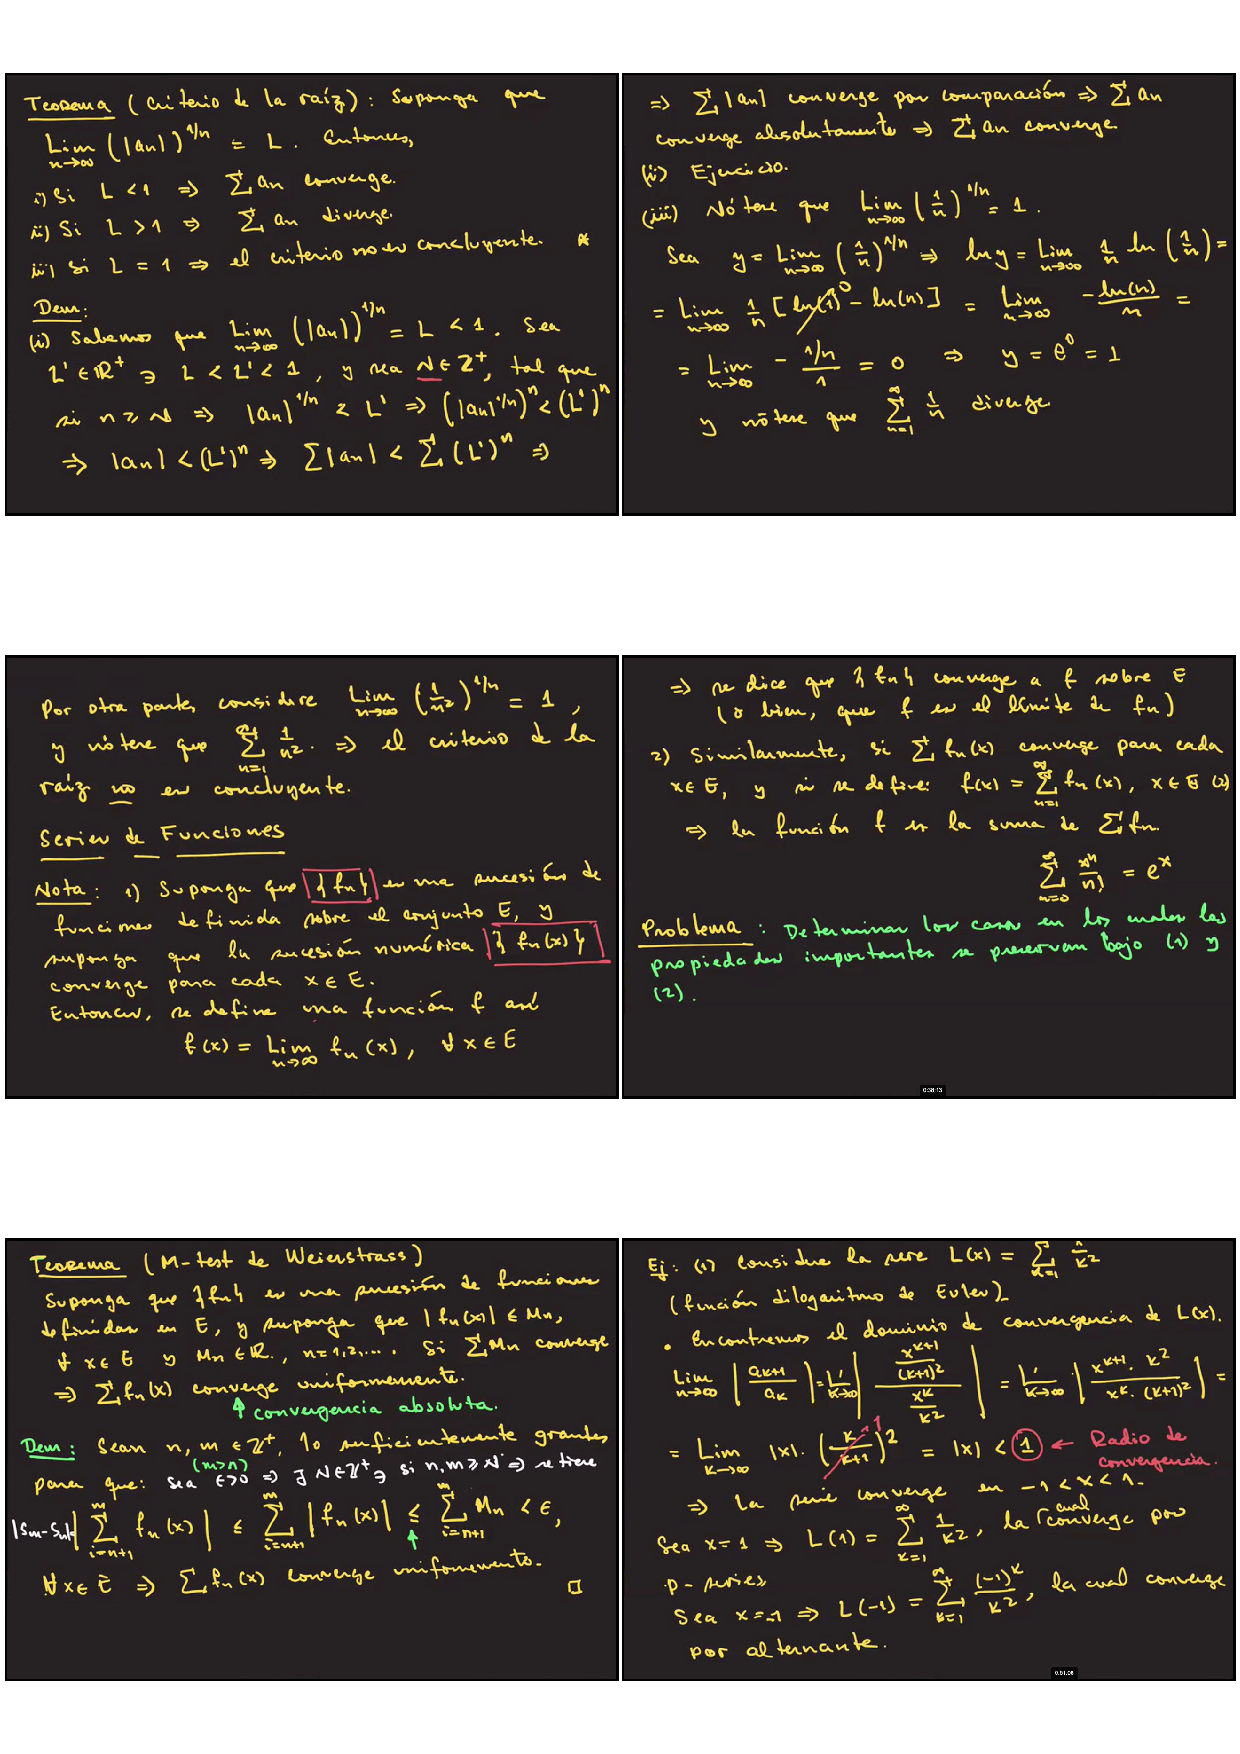
\includepdf[pages=-]{apendices/s14y15.pdf}